\documentclass[a4paper,12px]{article}
\usepackage{graphicx}
\usepackage[english]{babel}
\usepackage{fullpage}
\usepackage{xfrac}
\usepackage{fancyhdr}
\usepackage{lastpage}
\usepackage{xifthen}
\usepackage[linesnumberedhidden, titlenotnumbered]{algorithm2e}
\usepackage{lipsum}
\usepackage{hyperref}
\usepackage{array}
\usepackage{tabularx}
\usepackage{caption}
\usepackage{amsfonts}
\usepackage{amssymb}
\usepackage{amsmath}
\usepackage{mathtools}
\usepackage{placeins}
\usepackage{enumitem}
\usepackage[noabbrev]{cleveref}
\usepackage[utf8]{inputenc}
\usepackage{multirow}

\usepackage{minted}
\usepackage{listings}
\usepackage{dsfont}
\usepackage{units}

\pagestyle{fancy}
\lhead{
\includegraphics[width=7cm]{logoUvA}}
\rhead{\footnotesize \textsc {Report\\ \opdracht}}
\lfoot%
{%
    \footnotesize \studentA%
    \ifthenelse{\isundefined{\studentB}}{}{\\ \studentB}
    \ifthenelse{\isundefined{\studentC}}{}{\\ \studentC}
    \ifthenelse{\isundefined{\studentD}}{}{\\ \studentD}
    \ifthenelse{\isundefined{\studentE}}{}{\\ \studentE}
}
\cfoot{}
\rfoot{\small \textsc {Page \thepage\ of~\pageref{LastPage}}}
\renewcommand{\footrulewidth}{0.5pt}

\fancypagestyle{firststyle}
{%
    \fancyhf{}
    \renewcommand{\headrulewidth}{0pt}
    \chead{
\includegraphics[width=7cm]{logoUvA}}
    \rfoot{\small \textsc {Page \thepage\ of~\pageref{LastPage}}}
}

\setlength{\topmargin}{-0.3in}
\setlength{\textheight}{630pt}
\setlength{\headsep}{40pt}
\setlength{\parindent}{0pt}

% =================================== DOC INFO ===================================

\newcommand{\opdracht}{Theoretical Excercises}
\newcommand{\titel}{Labs week 3}
\newcommand{\docent}{Alban Ponse, Bob Diertens}
\newcommand{\cursus}{Theoretische aspecten van de Programmatuur}
\newcommand{\vakcode}{}
\newcommand{\datum}{\today}
\newcommand{\studentA}{Maico Timmerman}
\newcommand{\uvanetidA}{10542590}
%\newcommand{\studentB}{Tim van Zalingen}
\newcommand{\uvanetidB}{10784012}
% \newcommand{\studentC}{Boudewijn Braams}
\newcommand{\uvanetidC}{10401040}
% \newcommand{\studentD}{Govert Verkes}
\newcommand{\uvanetidD}{10211748}
%\newcommand{\studentE}{Naam student 5}
\newcommand{\uvanetidE}{UvAnetID student 5}

% ===================================  ===================================

\begin{document}
\thispagestyle{firststyle}
\begin{center}
    \textsc{\Large \opdracht}\\[0.2cm]
    \rule{\linewidth}{0.5pt} \\[0.4cm]
    {\huge \bfseries \titel}
    \rule{\linewidth}{0.5pt} \\[0.2cm]
    {\large \datum\\[0.4cm]}

    \begin{minipage}{0.4\textwidth}
        \begin{flushleft}

            \emph{Student:}\\
            {\studentA\\ {\small \uvanetidA\\[0.2cm]}}
            \ifthenelse{\isundefined{\studentB}}{}{\studentB\\ {\small \uvanetidB\\[0.2cm]}}
        \end{flushleft}
    \end{minipage}~%
    \begin{minipage}{0.4\textwidth}
        \begin{flushright}
            \emph{Lecturers:} \\
            \docent\\[0.2cm]
            \emph{Course:} \\
            \cursus\\[0.2cm]
            % \emph{Student:}\\
            \ifthenelse{\isundefined{\studentC}}{}{\studentC\\ {\small \uvanetidC\\[0.2cm]}}
            \ifthenelse{\isundefined{\studentD}}{}{\studentD\\ {\small \uvanetidD\\[0.2cm]}}
            \ifthenelse{\isundefined{\studentE}}{}{\studentE\\ {\small \uvanetidE\\ [0.2cm]}}
        \end{flushright}
    \end{minipage}\\[1 cm]
\end{center}


% =================================== CONTENTS ===================================

% \tableofcontents

\newcommand{\Sum}[2]{\sum^{#2}_{#1}}
\newcommand{\E}[1]{{\mathbb{E}\left[#1\right]}}
\newcommand{\var}[1]{{\text{var}\left[#1\right]}}
\newcommand{\diffpart}[1]{\frac{\partial}{\partial{} #1}}
\newcommand{\?}{\stackrel{?}{=}}
\newcommand{\intinf}{\int\limits_{-\infty}^{\infty}}
\newcommand{\intnulinf}{\int\limits_{0}^{\infty}}
\newcommand{\intpi}{\int\limits_{0}^{2\pi}}
\newcommand{\argmin}[1]{\underset{#1}{\mathop{\mathrm{argmin}}}}
\newcommand{\argmax}[1]{\underset{#1}{\mathop{\mathrm{argmax}}}}
\definecolor{bg}{rgb}{0.95,0.95,0.95}
% =================================== MAIN TEXT ===================================


\section{Factory}

The factory is started by creating the working cells and the channels.

\begin{minted}[bgcolor=bg]{C}
// Create all the new nodes.
wc1 = new;
wc2a = new;
wc2b = new;
wc3 = new;
input = new;
output = new;
channel12 = new;
channel13 = new;

// Create all value attributes for the nodes.
wc1.+v:str;
wc2a.+v:str;
wc2b.+v:str;
wc3.+v:str;
channel12.+v:str = "";
channel13.+v:str = "";

// Connect working cell 1 (wc1) to working cell 2 (wc2) using channel12.
wc1.+a = channel12;
channel12.+a2 = wc2a;
channel12.+a1 = wc2b;

// Connect working cell 1 (wc1) to working cell 3 (wc3) using channel12.
wc1.+b = channel13;
channel13.+b = wc3;

// Set the initial queue's for in- and output.
input.+q:str = "ABAB";
output.+q:str = "";

// Connect input and output.
input.+ab = wc1;
wc2a.+a = output;
wc2b.+a = output;
wc3.+b = output;
\end{minted}

\begin{figure}[h]
    \centering
    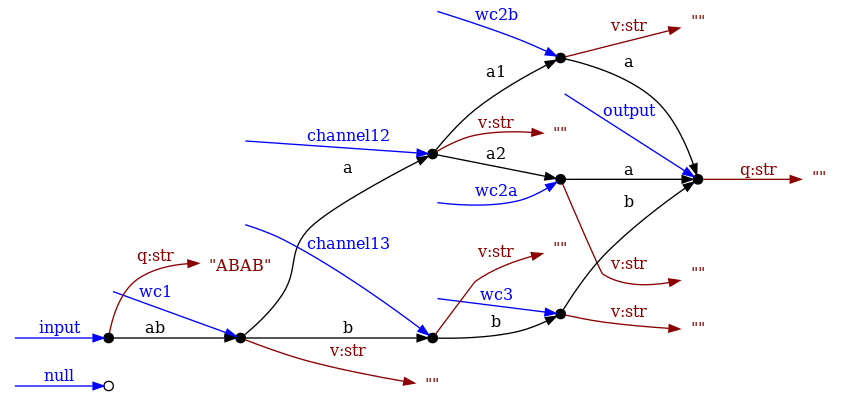
\includegraphics[width=0.8\linewidth]{factory.png}
    \caption{Fluid of factory using 3 working cells and 2 instances of wc2.}
    \label{fig:factory}
\end{figure}
\FloatBarrier%

After creating the fluid for the factory, the threads are spawned. Labeled jumps  are used to jump to the correct code.

\begin{minted}[bgcolor=bg]{C}
// Spawn working cell 1 (wc1) thread.
fork #2;
##L1;

// Spawn working cell 2 (wc2) thread.
fork #2;
##L2;

// Spawn another working cell 2 (wc2) thread.
fork #2;
##L22;

// Use the left-over thread for working cell 3 (wc3)
##L3;
\end{minted}

The thread for working cell 1 (wc1) takes input from the \verb|input| and
passes all \verb|A|'s  to working cell 2(wc2) and \verb|B|'s to working cell 3
(wc3). To take or put something into a shared resource, a lock is used. A lock
is created using the field introduction instruction. Specifically, using this
instruction as a test instruction. By testing if \verb|lock| can be created, we
have an atomic instruction to lock the focus.
\begin{figure}[h]
    \centering
    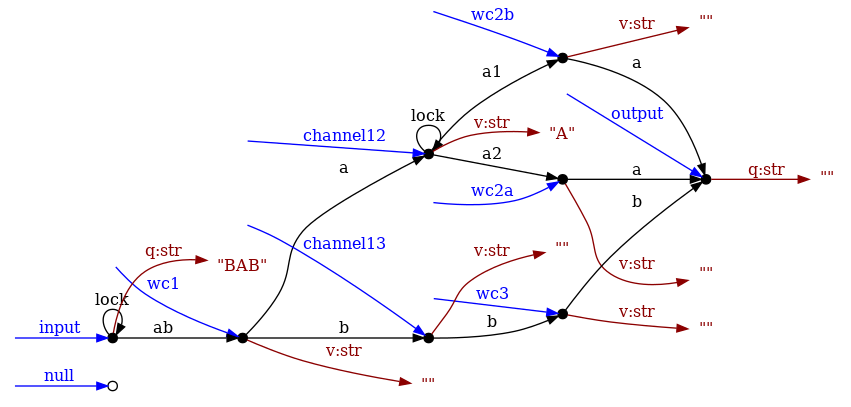
\includegraphics[width=0.8\linewidth]{lock.png}
    \caption{Example of locking in action.}
    \label{fig:lock}
\end{figure}
\FloatBarrier%

\begin{minted}[bgcolor=bg]{C}
L1;
// Determine offloading/loading.
+wc1.v==""{;
    // Try to fetch lock for input, if it fails, restart thread.
    -input.+lock; ##L1;

    // Test if there is something in the input.
    +input.v==""{;
    }{;
        // Load the first value into the working cell and remove from input.
        first input.q wc1.v;
        delfirst input.q;
    };
    // Unlock and restart.
    input.-lock;
    ##L1;
}{;
    // 'A' values need to be passed to channel12.
    +wc1.v=="A"{;
        // Try to fetch lock for channel12, it it fails, restart thread.
        -channel12.+lock; ##L1;
        +channel12.v==""{;
            first wc1.v channel12.v;
            delfirst wc1.v;
        }{;
        };
        // Unlock and restart.
        channel12.-lock;
        ##L1;
    }{;
    };

    // 'B' values need to be passed to channel13.
    +wc1.v=="B"{;
        // Try to fetch lock for channel13, it it fails, restart thread.
        -channel13.+lock; ##L1;
        +channel13.v==""{;
            // Load the first value into the working cell and remove from channel.
            first wc1.v channel13.v;
            delfirst wc1.v;
        }{;
        };
        // Unlock and restart.
        channel13.-lock;
        ##L1;
    }{;
    };
    ##L1;
};
\end{minted}

Code for working cell 2 (wc2) is very similar to the code of working cell 1
(wc1). When the addition wc2 cell was spawned, the code was duplicated and
\verb|wc2a| was replaced with \verb|wc2b|, however the inner working is exactly
the same. For working cell 3 (wc3) the code is also the same, however it works
with \verb|channel13| and \verb|wc3|.

\begin{minted}[bgcolor=bg]{C}
L2;
+wc2a.v==""{;
    // Check if there are values in channel12, if not, restart thread.
    +channel12.v==""; ##L2;
    // Try to fetch lock for channel12, it it fails, restart thread.
    -channel12.+lock; ##L2;
    +channel12.v==""{;
    }{;
        // Move value from channel12 to working cell.
        first channel12.v wc2a.v;
        delfirst channel12.v;
    };
    // Unlock and restart.
    channel12.-lock;
    ##L2;
}{;
    // Try to fetch lock for output, it it fails, restart thread.
    -output.+lock; ##L2;

    // Move value from working cell to end of output.
    append output.q wc2a.v;
    delfirst wc2a.v;

    // Unlock and restart.
    output.-lock;
    ##L2;
};

\end{minted}

% =================================== REFERENCES ===================================

% \clearpage

% \bibliographystyle{apalike}
% \bibliography{report}

\end{document}
